\documentclass[12pt]{jhwhw}
\author{Ian Malerich}
\title{Com S 352: Homework 3}
\usepackage{amssymb, amsfonts, mathtools, graphicx, breqn}
\usepackage{minted, subfig, float, scrextend, setspace, soul}
\usemintedstyle{friendly}

\onehalfspacing
\begin{document}
\raggedright

%% Problem 4.8
\textbf{4.8 (8 points)}  Which of the following components of program state are 
	shared across threads in a multithreaded process.
	\begin{enumerate}
		\item Register Values
		\item Heap Memory
		\item Global Variables
		\item Stack Memory
	\end{enumerate}
\textcolor[RGB]{240,240,240}{\rule{\textwidth}{0.5pt}}\bigbreak

	\begin{addmargin}[1em]{}
		\hl{Heap Memory} and \hl{Global Variables} are shared between threads in a 
		multithreaded process. 
		Both the stack and registers are needed for executing the separate
		paths of code, and thus will not be shared.
	\end{addmargin}
	\bigbreak

%% Problem 4.11
\textbf{4.11 (5 points)} Is it possible to have concurrency but not parallelism?
	Explain.
\textcolor[RGB]{240,240,240}{\rule{\textwidth}{0.5pt}}\bigbreak

	\begin{addmargin}[1em]{}
		Yes. Parallelism requires multiple CPU's, so that multiple processes/threads
		are being run simultaneously in real time. Concurrency only requires that more
		than one process/thread is in the process of being computed at a time, thus,
		multiple process/thread may share a single CPU (not parallel) and alternate
		turns executing code by following some scheduling algorithm.
	\end{addmargin}
	\bigbreak

%% Problem 4.17
\textbf{4.17 (10 points)} The program shown below uses the pthreads API. 
	What would be the output from the program at LINE C and LINE P?
\inputminted{c}{4.17.c}
\textcolor[RGB]{240,240,240}{\rule{\textwidth}{0.5pt}}\bigbreak

	\begin{addmargin}[1em]{}
		The parent process creates a new child process, this child process
		then  creates a new thread. The parent and the child have entirely separate
		memory spaces, where the child and it's created thread share some memory
		as detailed in problem 4.8, this happens to include 'value'.
		The 'value' is only changed by the process created by the child, thus,
		as the child waits for this process to finish via
		pthread_join, \hl{LINE C} will output a value of \hl{5} (set by the thread).
		However, this all happens outside of the parents memory, thus it will be unchanged.
		Therefore \hl{LINE P} will output a value of \hl{0}.
	\end{addmargin}
	\bigbreak

\clearpage
%% Problem 6.14
\textbf{6.14 (15 points)} Consider the exponential average formula used to
	predict the length of the next CPU burst. What are the implications of assigning
	the values to the parameters used by the algorithm?
	\begin{enumerate}
		\item $\alpha=0$ and $\tau_0=100$ ms
		\item $\alpha=0.99$ and $\tau_ 0=10$ ms
	\end{enumerate}
\textcolor[RGB]{240,240,240}{\rule{\textwidth}{0.5pt}}\bigbreak

	\begin{addmargin}[1em]{}
		\begin{enumerate}
			\item $(\alpha=0,\tau_0=100)$ \\
				$\tau_{n+1} = \alpha\times t_n + (1-\alpha)\tau_n$ \\
				$\tau_{n+1} = 0\times t_n + \tau_n$ \\
				$\tau_{n+1} = \tau_n$ \\
				Note that we have killed off $t_i$ the actual length of
				the $i^{th}$ CPU burst. Thus, the prediction will always be
				equivalent to the last prediction ($\tau_n$).
				Therefore, this algorithm will always estimate a constant
				CPU burst time of $100$ms regardless of process.

			\item $(\alpha=0.99,\tau_0=10)$ \\
				$\tau_{n+1} = \alpha\times t_n + (1-\alpha)\tau_n$ \\
				$\tau_{n+1} = 0.99\times t_n + 0.01\tau_n$ \\
				Here we see the algorithm very heavily weighted in favor of $t_n$, the 
				actual length of the last CPU burst. Thus, this algorithm will
				fluctuate easily. For example, if a process has many short CPU bursts,
				but then one long one, for the following burst estimate, 
				the algorithm will mostly ignore the last estimate
				(which would have been short) and go with a long estimate, very close
				to the last CPU burst time ($t_n$), even though we would assume given
				the long term behavior of the process, a short burst would be more likely.
		\end{enumerate}
	\end{addmargin}
	\bigbreak

%% Problem 6.16
\textbf{6.16 (30 points)} 
	Consider the following set of processes, with the length of the CPU
	burst given in milliseconds: \\
	\begin{centering}
	\begin{tabular}{| l | c | c | c | c | c |}
		\hline
		Process & P1 & P2 & P3 & P4 & P3 \\
		\hline
		Burst Time & 2 & 1 & 8 & 4 & 5 \\
		\hline
		Priority & 2 & 1 & 4 & 2 & 3 \\
		\hline
	\end{tabular} \\
	\end{centering}
	\bigbreak
	The processes are assumed to have arrived in the order P1, P2, P3, P4, P5, all at 
	time 0.
	\begin{enumerate}
		\item Draw four Gantt charts that illustrate the execution of these processes using the
			following scheduling algorithms: FCFS, SJF, non-preemptive priority (a larger
			priority number implies a higher priority), and RR (quantum = 2).
		\item What is the turnaround time of each process for each of the scheduling algorithms
			in part a?
		\item What is the waiting time of each process for each of these scheduling algorithms.
		\item Which of the algorithms results in the minimum average waiting time
			(over all processes)?
	\end{enumerate}
\textcolor[RGB]{240,240,240}{\rule{\textwidth}{0.5pt}}\bigbreak

	\textbf{(a)} \\
	\begin{centering}
	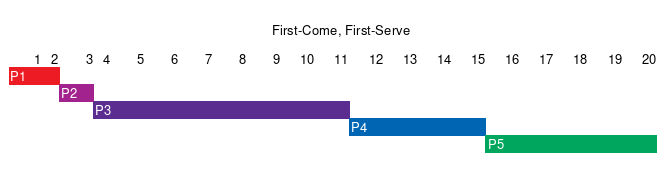
\includegraphics[scale=0.65]{fcfs.png} \\
	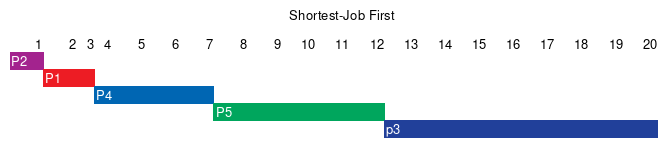
\includegraphics[scale=0.65]{sjf.png} \\
	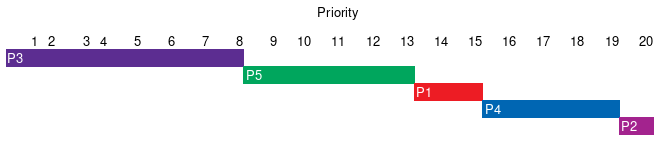
\includegraphics[scale=0.65]{prio.png} \\
	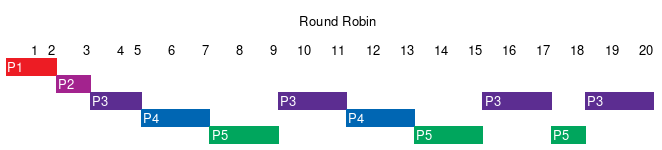
\includegraphics[scale=0.65]{rr.png} \\
	\end{centering}
	\clearpage

	\begin{addmargin}[1em]{}
		\textbf{(b)} \\
		\begin{centering}
		\begin{tabular}{| l | c | c | c | c | c |}
			 \hline
			     & P1 & P2 & P3 & P4 & P5 \\
			 \hline
			First-Come, First Serve & 2 & 1 & 8 & 4 & 5 \\
			\hline
			Shortest-Job First & 2 & 1 & 8 & 4 & 5 \\
			\hline
			Priority & 2 & 1 & 8 & 4 & 5 \\
			\hline
			Round Robin & 2 & 1 & 17 & 8 & 11 \\
			\hline
		\end{tabular} \\
		\end{centering}
		\bigbreak
		From the graphs, we can clearly see that Round Robin is the only
		method which interrupts execution of a process, thus for FCFS, SJF, and
		Priority, the turn around times are equivalent to the CPU burst time.
		Round Robin however has much longer turn around times as long process
		are evenly distributed over the entire execution time.

		\textbf{(c)} \\
		\begin{centering}
		\begin{tabular}{| l | c | c | c | c | c |}
			 \hline
			     & P1 & P2 & P3 & P4 & P5 \\
			 \hline
			First-Come, First-Serve & 0 & 2 & 3 & 11 & 15 \\
			\hline
			Shortest-Job First & 1 & 0 & 12 & 3 & 7 \\
			\hline
			Priority & 13 & 19 & 0 & 15 & 8 \\
			\hline
			Round Robin & 0 & 2 & 11.25 & 8 & 12.33 \\
			\hline
		\end{tabular} \\
		\end{centering}

		\textbf{(d)} \\
		\begin{centering}
		\begin{tabular}{| c | c | c | c |}
			\hline
			FCFS & Shortest-Job First & Priority & Round Robin \\
			\hline
			6.2 & 4.6 & 11 & 6.716 \\
			\hline
		\end{tabular} \\
		\end{centering}
		\bigbreak
		In the table of average wait times above (the sum of each row in part (c) divided
		by 5), we see that Shortest Job First has the smallest wait time, which is as 
		expected. Leaving long jobs for the end minimizes the wait time for all 
		processes and is the primary strength of the SJF algorithm.

	\end{addmargin}
	\bigbreak

%% Problem 6.19
\textbf{6.19 (5 points)} 
	Which of the following scheduling algorithms could result in starvation?
	\begin{enumerate}
		\item First-Come, First-Served
		\item Shortest Job First
		\item Round Robin
		\item Priority
	\end{enumerate}
\textcolor[RGB]{240,240,240}{\rule{\textwidth}{0.5pt}}\bigbreak

	\begin{addmargin}[1em]{}
		\hl{Priority} can, if you have a process with low priority, and new process
		constantly filter in with high priority as other process complete, these
		new processes will always take control of the CPU over the low priority process.
		Thus starvation occurs and the low priority process is never executed.
		\bigbreak
		In a similar manner, \hl{Shortest Job First} could also create starvation,
		where instead of a low priority process, we have a long job, then
		as short jobs are completed, more process are introduced with short CPU
		requirements. These short processes will continue to grab the CPU, and the
		long job process will be starved.
		\bigbreak
		FCFS guarantees that all process will eventually receive the CPU (by the order
		they come in), Round Robin is treats all processes equally and constantly
		switches between them, thus all processes will eventually be processed.
	\end{addmargin}
	\bigbreak

%% Problem 6.23
\textbf{6.23 (7 points)} 
	Consider a preemptive priority scheduling algorithm based on dynamically
	changing priorities. Larger priority numbers imply higher priority.
	When a process is waiting for the CPU (in the ready queue, but not
	running), its priority change at a rate $\alpha$. When it is running, its
	priority changes at a rate $\beta$. All processes are given a priority of 0 when they
	enter the ready queue. The parameters $\alpha$ and $\beta$ can be set to give 
	many different scheduling algorithms.
	\begin{enumerate}
		\item What is the algorithm that results from $\beta > \alpha > 0$?
		\item What is the algorithm that results from $\alpha < \beta < 0$?
	\end{enumerate}
\textcolor[RGB]{240,240,240}{\rule{\textwidth}{0.5pt}}\bigbreak

	\begin{addmargin}[1em]{}
		\begin{enumerate}
			\item
				First-Come, First-Serve \\
				The instant a process starts running, it will have the highest priority,
				as $\beta > \alpha > 0$ the priority will continue to increase at a rate
				greater than any process, thus it will have the highest priority 
				and will continue to execute until completion. \\
				For processes in the queue, processes who have been waiting longer 
				(first come) will have higher priority (first serve) than newer processes
				in the queue.
			\item
				Last-In, First-Out \\
				As $\alpha < \beta < 0$, processes in the queue will always
				have lower priority than any running priority. Further, as 
				running process lose priority slower, running processes will never
				be interrupted by processes currently in queue. However, any new process
				with priority 0 will automatically have a higher priority than the running
				process and will preempt that process pushing it back to the queue 
				(where it will maintain highest priority in queue).
				Thus, newest processes (Last-In), will be the first to be executed 
				(First-Out), and will only complete if no new process is added
				during their execution.
		\end{enumerate}
	\end{addmargin}

%% Problem 7
\textbf{7 (20 points)} Convert the following program to use threads.
	Under the following restrictions:
	\begin{enumerate}
		\item One thread will print ``hello", one thread will print ``world", and the
			main function will print the trailing $``\backslash n"$, using just
			pthread_create(), pthread_exit(), pthread_yield(), and
			pthread_join().
		\item You must use a synchronization method to ensure the "world" thread
			runs after the "hello" thread.
		\item You must use a synchronization method to ensure that the main
			thread does not execute until after the "world" thread.
	\end{enumerate}

\textcolor[RGB]{240,240,240}{\rule{\textwidth}{0.5pt}}\bigbreak
\inputminted{c}{7.c}

\end{document}
